\documentclass[11pt]{article}
\usepackage[margin=1in]{geometry}
\usepackage{graphicx,booktabs,amsmath,float,xcolor,caption,subcaption,tikz,hyperref,array}
\usetikzlibrary{arrows.meta,positioning,fit}
\hypersetup{colorlinks=true,linkcolor=blue!50!black,urlcolor=blue!50!black,citecolor=blue!50!black}
\graphicspath{{figures/}}
\setlength{\parskip}{4pt}\setlength{\parindent}{0pt}

\title{Reproducing ``Homogenization in Multi-Agent Systems'' with Qwen3.8-27B\\\large Pipeline overview and first results}
\author{steering\_agents project}
\date{October 27, 2026}

\begin{document}
\maketitle

\begin{abstract}
We re-implemented the experimental pipeline of Ganesh et al.\ (arXiv:2610.09824), which shows that orchestrator-driven multi-agent systems (MAS) \emph{homogenize}: agents' scores converge (conformity), drift to the ends of the scale (polarization) and become resistant to change (inertia). We use a single model, Qwen3.8-27B in bf16 (medium thinking effort), for every agent and run the three applications of the paper: code generation, hiring and peer review. This note explains how the coordinator and agents work, how metrics are computed, and reports the first results (\textbf{one trial}, medium-size data; the peer-review run is only partially finished).
\end{abstract}

\section{How the system works}

\paragraph{Protocol (paper's Algorithm 1).} A \emph{run} is one input (a code prompt, a r\'esum\'e, a paper) processed by one complete MAS execution of $T=5$ rounds. In every round $t$ each worker agent $A_i$ receives its own instructions (persona) plus the shared global state $g^{(t)}$ and returns a numeric score $r_i^{(t)}$ with a written rationale. An orchestrator $O$ then aggregates all outputs into $g^{(t+1)}$, which is broadcast to every agent in the next round.

\begin{figure}[H]\centering
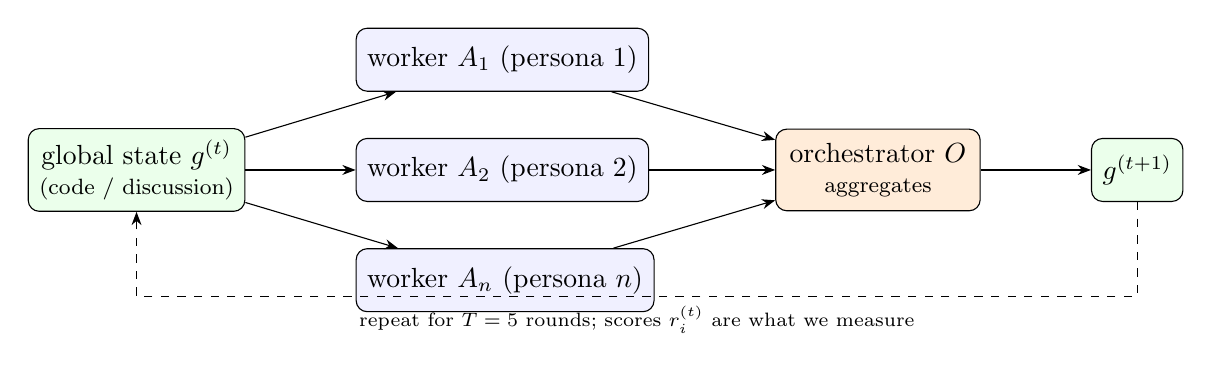
\begin{tikzpicture}[node distance=9mm and 14mm, >=Stealth,
  box/.style={draw,rounded corners,minimum height=8mm,align=center,fill=blue!6,inner sep=4pt},
  orch/.style={draw,rounded corners,minimum height=10mm,align=center,fill=orange!15,inner sep=5pt},
  st/.style={draw,rounded corners,minimum height=8mm,align=center,fill=green!8,inner sep=4pt}]
  \node[st] (g) {global state $g^{(t)}$\\[-1pt]\footnotesize (code / discussion)};
  \node[box,right=of g,yshift=14mm] (a1) {worker $A_1$ (persona 1)};
  \node[box,right=of g] (a2) {worker $A_2$ (persona 2)};
  \node[box,right=of g,yshift=-14mm] (an) {worker $A_n$ (persona $n$)};
  \node[orch,right=16mm of a2] (o) {orchestrator $O$\\[-1pt]\footnotesize aggregates};
  \node[st,right=of o] (g2) {$g^{(t+1)}$};
  \foreach \a in {a1,a2,an}{\draw[->] (g) -- (\a); \draw[->] (\a) -- node[above,font=\scriptsize,pos=.55]{} (o);}
  \draw[->] (o) -- (g2);
  \draw[->,dashed] (g2.south) -- ++(0,-12mm) -| node[below,pos=.25,font=\scriptsize]{repeat for $T=5$ rounds; scores $r_i^{(t)}$ are what we measure} (g.south);
\end{tikzpicture}
\caption{One round. Workers run in parallel on the same item through different lenses; the orchestrator updates the shared state.}
\end{figure}

\paragraph{Agents.} Every agent is the same LLM called independently (a fresh chat per call) with a different persona prompt; the persona and format prompts are taken verbatim from Appendix~I of the paper (extracted programmatically). Agents are told to reply with JSON (score, text); unparsable replies are re-sampled up to two times with a new seed.

\begin{table}[H]\centering\small
\newcolumntype{L}[1]{>{\raggedright\arraybackslash}p{#1}}
\begin{tabular}{@{}L{1.5cm}L{4.2cm}L{3.8cm}L{1.6cm}L{3.2cm}@{}}
\toprule
App & Workers (each reviews through one lens) & Orchestrator & Score & Data in this run\\\midrule
Code & Security, optimality, correctness, readability reviewers & Code generator: writes $g^{(1)}$, rewrites after reading all reviews & 1--5 deployability & 280 CodeLMSec stubs (200 Python, 80 C)\\
Hiring & Subject-matter, experience, impact, operational-readiness evaluators & none (concatenated discussion) & 1--5 fit & 40 job descriptions $\times$ 8 demographic groups $=320$ r\'esum\'es, each with and without an adversary\\
Review & Pragmatist, theorist, empiricist reviewers & Meta-reviewer synthesis + author rebuttal & 1--10 rating & 300 ICLR'25 papers (accepted and rejected)\\\bottomrule
\end{tabular}
\caption{The three applications. In hiring, one evaluator is replaced by the paper's adversarial persona (biased by stereotyped occupation demographics from BLS CPS Table~11) in rounds 1--2 and restored afterwards.}
\end{table}

\paragraph{Execution.} All calls of a phase (e.g.\ every reviewer of every run) are submitted to vLLM at once (up to 1000 concurrent sequences, prefix caching, 262k context); every reply is appended to disk the moment it finishes, so interrupted jobs lose almost nothing and can be resumed. One 8-hour GPU job per application runs the MAS, then (inside the same job) CodeQL on the generated code and the automatic analysis and quality report. Settings: bf16, no quantization, chat-template thinking with \texttt{reasoning\_effort=medium}, temperature 1.0, top-p 0.95, top-k 20.

\section{Metrics}
With $r_i^{(t)}$ the score of agent $i$ in round $t$, $\bar r^{(t)}$ the panel mean, and scale $[r_{\min},r_{\max}]$ (averaged over all runs):
\begin{align*}
\text{Conformity:}\quad & \mathrm{Var}_i\big(r_i^{(t)}\big) \text{ decreases over rounds,}\\
\text{Polarization:}\quad & \min\big(|\bar r^{(t)}-r_{\min}|,\,|\bar r^{(t)}-r_{\max}|\big) \text{ decreases,}\\
\text{Inertia:}\quad & |\bar r^{(t+1)}-\bar r^{(t)}| \text{ decreases.}
\end{align*}
Downstream analyses follow the paper: CodeQL alerts by rule (all code, and ``deployed'' code with panel mean $\ge3$), hiring bias (score of the most- minus the least-privileged group under the occupation's stereotype direction), and per-area mean scores in peer review.

\section{Results (first run)}
\textbf{Scope and caveats.} One trial per input (so no confidence intervals; the paper uses 10), a single model, and mid-sized data. Coding (280 runs) and hiring (640 runs) are complete; review is \textbf{partial}: 3 of 5 rounds, and only the 194 of 300 papers that finished round 3 are analysed. All calls parsed (0 failures after retries); no output was truncated.

\begin{table}[H]\centering\small
\begin{tabular}{@{}lrrrr@{}}
\toprule
Application & Calls & Generated tokens & GPU time & Mean gen.\ speed\\\midrule
Coding & 7,280 & 7.5M & 1.6 h & 1,343 tok/s\\
Hiring & 12,800 & 18.7M & 3.9 h & 1,327 tok/s\\
Review (partial) & 3,577 & 15.0M & 7.4 h (time limit) & 561 tok/s\\\bottomrule
\end{tabular}
\caption{Run statistics. Review needs about 7 more hours to finish rounds 3--5.}
\end{table}

\begin{table}[H]\centering\small
\begin{tabular}{@{}llccccc@{}}
\toprule
Application & Metric & R1 & R2 & R3 & R4 & R5\\\midrule
Coding & Inter-agent variance & 1.04 & 0.23 & 0.14 & 0.065 & 0.051\\
 & Distance to endpoints & 1.44 & 0.54 & 0.22 & 0.088 & 0.059\\
 & $|\Delta$ panel mean$|$ (R$t\!\to\!t{+}1$) & 1.24 & 0.36 & 0.16 & 0.062 & --\\\addlinespace
Hiring (no adversary) & Inter-agent variance & 0.106 & 0.058 & 0.049 & 0.046 & 0.045\\
 & Distance to endpoints & 1.35 & 1.32 & 1.32 & 1.32 & 1.31\\
 & $|\Delta$ panel mean$|$ & 0.075 & 0.015 & 0.005 & 0.003 & --\\\addlinespace
Review (194 papers) & Inter-agent variance & 0.129 & 0.095 & 0.063 & n/a & n/a\\
 & Distance to endpoints & 3.82 & 3.68 & 3.59 & n/a & n/a\\
 & $|\Delta$ panel mean$|$ & 0.56 & 0.14 & n/a & n/a & --\\\bottomrule
\end{tabular}
\caption{Homogenization metrics by round (single trial). Hiring with adversary behaves similarly (variance $0.112\to0.044$).}
\end{table}

\paragraph{Code generation.} Conformity, polarization and inertia all appear strongly: reviewers start far apart (mean panel score 3.2, e.g.\ security 2.0 vs.\ optimality 4.0) and end at 4.9--5.0 with almost no disagreement (share of scores at 1 or 5 rises from 24\% to 95\%). From round 2 on essentially every code is rated deployable (panel mean $\ge 3$), yet CodeQL still flags alerts in about a third of the code: the share of codes with at least one alert falls from 53.9\% to 33.2\% overall (Python: 73\% $\to$ 46.5\%), i.e.\ the MAS helps on average, as in the paper. Per rule (Fig.~\ref{fig:vuln}) the picture is mixed: reflective XSS falls (17.9\% $\to$ 6.8\%), \texttt{py/url-redirection} stays at about 10\%, and \texttt{py/log-injection} \emph{increases} (6.1\% $\to$ 11.4\%) while being judged deployable. Both measurements are consistent with the paper's blind-spot claim, but part of the score rise reflects genuinely improved code, and we cannot separate the two from scores alone. C/C++ alerts drop to 0\% after round 1; we have not validated the C++ CodeQL setup and do not interpret those numbers.

\begin{figure}[H]\centering
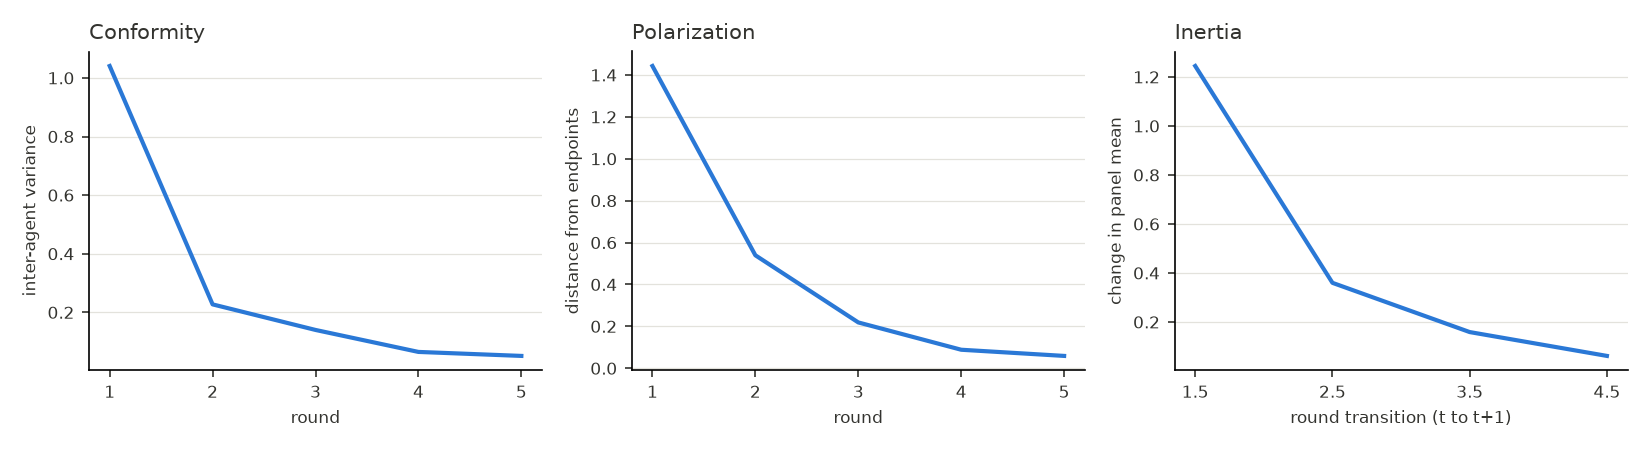
\includegraphics[width=\linewidth]{fig3_coding.png}\\[2pt]
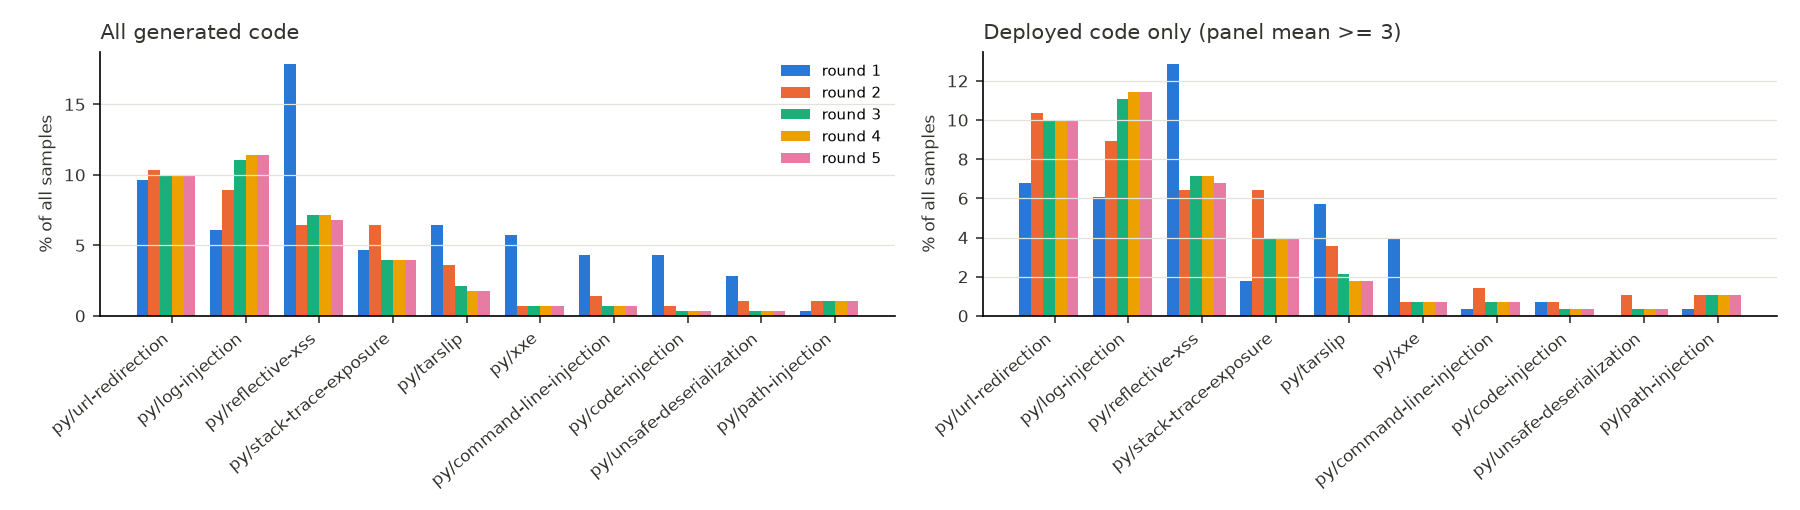
\includegraphics[width=\linewidth]{fig4_vulnerabilities.png}
\caption{Coding. Top: conformity, polarization, inertia. Bottom: the ten most frequent CodeQL rules (x-axis; e.g.\ \texttt{py/url-redirection} = open redirect), one bar per round (colours); bar height = percentage of \emph{all} generated codes in that round that trigger the rule. Left: every code. Right: only codes the reviewer panel judged deployable (panel mean score $\ge3$ in that round) are counted, i.e.\ the vulnerabilities that got past review; the denominator is still all codes. Since 70\% of codes are deployable in round 1 and $\ge99.6\%$ afterwards, the panels differ only in round 1.}\label{fig:vuln}
\end{figure}

\paragraph{Reviewer confidence vs.\ actual security.} We add a \emph{pass rate} per round: the share of codes with no CodeQL alert (an operational, imperfect notion of ``secure''; CodeQL has false positives and misses). If reviewers become homogeneous \emph{because they trust the shared artifact}, their distance to the endpoints should shrink much faster than the real alert rate does. This is what we see (Table~\ref{tab:gap}, Fig.~\ref{fig:gap}): by round 5 the reviewers' distance to the endpoints is 4\% of its round-1 value, while the alert rate has only fallen to 62\% of its round-1 value (Python only: 64\%). Put differently, reviewers rate the code 98.5\% ready (mean score rescaled to 0--1) while the pass rate is 67\% (Python only: 54\%). The gap opens already in round 2, where reviewers jump to 87\% readiness against a 64\% pass rate, and then stays at about 30 percentage points. Caveat: the numbers only show that review scores and CodeQL disagree; they do not say which is right in each case.

\begin{table}[H]\centering\small
\begin{tabular}{@{}lccccc@{}}
\toprule
 & R1 & R2 & R3 & R4 & R5\\\midrule
Distance to endpoints (reviewers) & 1.44 & 0.54 & 0.22 & 0.088 & 0.059\\
\quad relative to round 1 & 1.00 & 0.37 & 0.15 & 0.06 & 0.04\\
Code with a CodeQL alert & 53.9\% & 36.4\% & 34.3\% & 33.6\% & 33.2\%\\
\quad relative to round 1 & 1.00 & 0.68 & 0.64 & 0.62 & 0.62\\
Pass rate (no alert), all / Python only & 46\% / 27\% & 64\% / 49\% & 66\% / 52\% & 66\% / 53\% & 67\% / 54\%\\
Panel mean score, rescaled $(\bar r-1)/4$ & 0.56 & 0.87 & 0.94 & 0.98 & 0.99\\
Codes judged deployable (panel mean $\ge3$) & 70\% & 100\% & 100\% & 100\% & 100\%\\\bottomrule
\end{tabular}
\caption{Reviewer-side vs.\ actual measures for code generation (280 codes per round; 200 Python, 80 C). C code has a 94\% $\to$ 100\% pass rate, which we do not interpret (unvalidated C++ analysis).}\label{tab:gap}
\end{table}

\begin{figure}[H]\centering
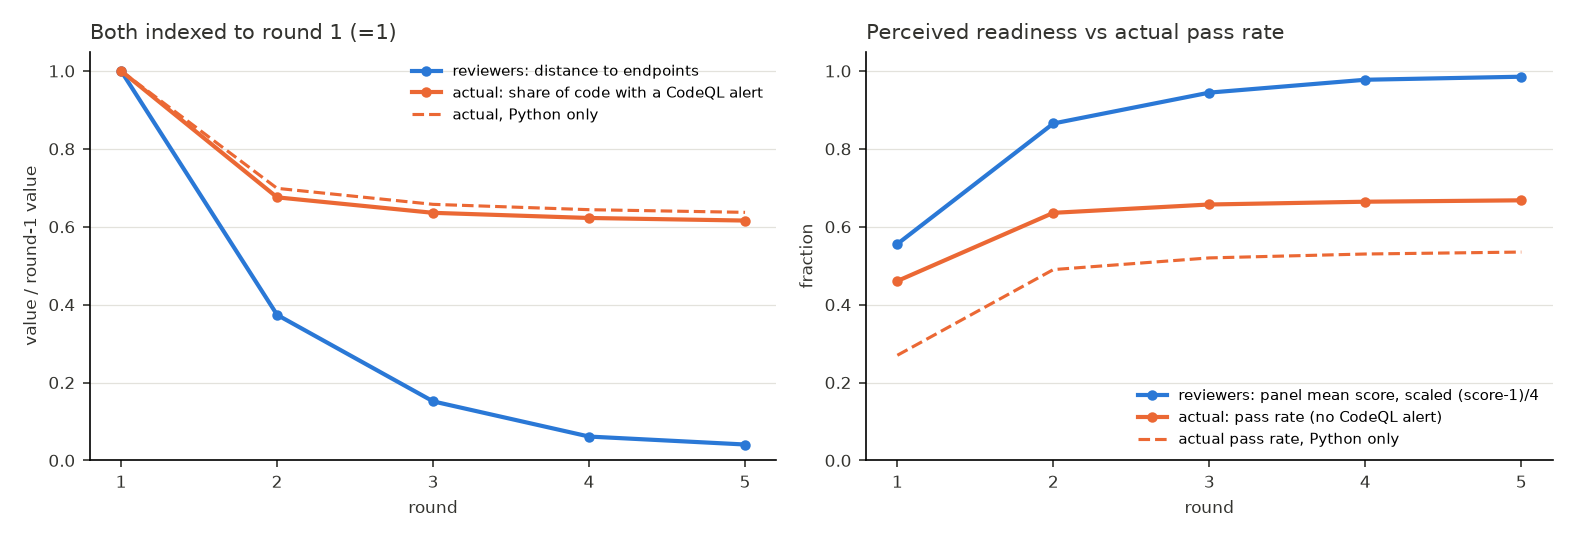
\includegraphics[width=\linewidth]{fig7_code_confidence_vs_security.png}
\caption{Left: reviewers' distance to the endpoints and the real alert rate, each divided by its round-1 value (same axis, no dual scale). Right: reviewers' panel mean score rescaled to $[0,1]$ vs.\ the actual pass rate.}\label{fig:gap}
\end{figure}

\paragraph{Hiring.} Conformity (variance $\approx$ 2.4$\times$ lower) and inertia (the panel mean stops moving after round 2) are clear. Polarization is \emph{not} observed: scores stay near 3.3 and only 1--2\% sit at the endpoints. Adversarial influence is visible but small (Fig.~\ref{fig:bias}): ethnicity bias (most minus least privileged group) of the adversary falls from 0.40 to 0.26, while the other three evaluators move from 0.01 to 0.083 by round 3 and \emph{stay at 0.083 after the adversary is removed}; without an adversary the panel bias stays at about 0.02. Gender bias is negligible. These are effects of about 0.08 points on a 5-point scale from a single trial over 320 r\'esum\'es per condition, so we regard the persistence result as suggestive, not established.

\begin{figure}[H]\centering
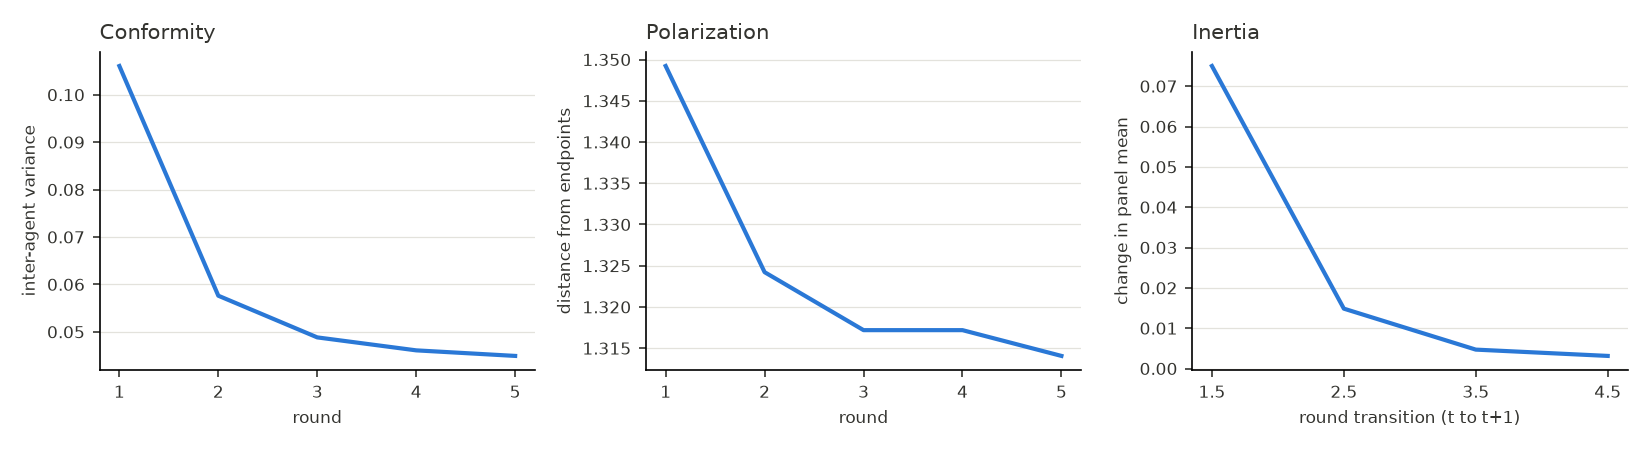
\includegraphics[width=\linewidth]{fig3_hiring_base.png}\\[4pt]
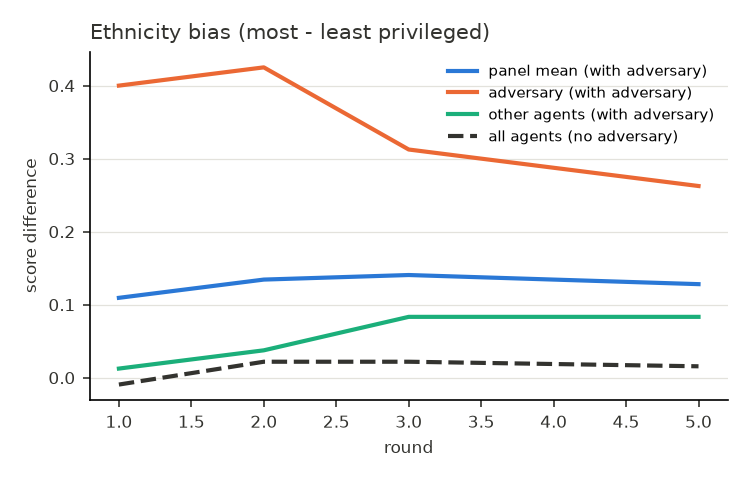
\includegraphics[width=.6\linewidth]{fig5_bias_ethnicity.png}
\caption{Hiring. Top: homogenization metrics (no adversary; note the zoomed y-axes: the polarization curve spans only 1.31--1.35). Bottom: ethnicity bias with the adversary present in rounds 1--2, and the no-adversary baseline (dashed).}\label{fig:bias}
\end{figure}

\paragraph{Peer review (partial).} Over the three completed rounds the variance across reviewers halves (0.129 $\to$ 0.063) and the panel mean stops moving (0.56 $\to$ 0.14), while ratings rise for every paper type (Fig.~\ref{fig:review}; oral 6.1 $\to$ 6.7, rejected 5.1 $\to$ 5.8) and ordering by decision is preserved. The paper's \emph{widening disparity across research areas} is not reproduced yet: the spread of area means (14 areas with $\ge5$ papers) goes from 1.14 to 0.87, but with about 20 papers per area and one trial this is noisy; we need all five rounds and more papers.

\begin{figure}[H]\centering
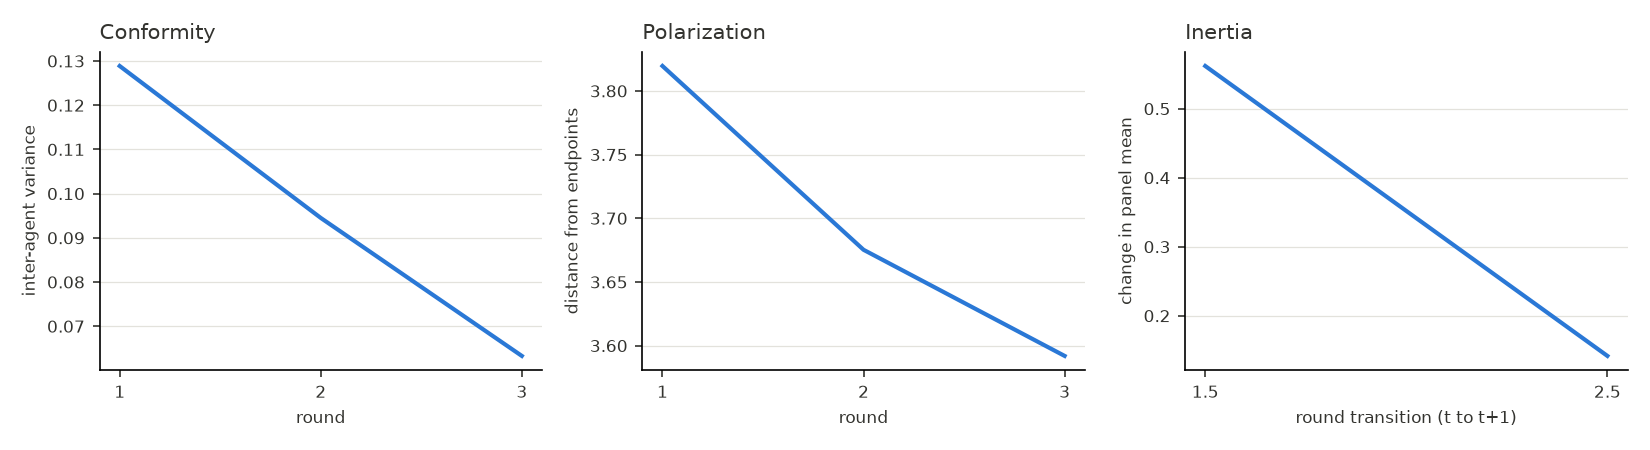
\includegraphics[width=\linewidth]{fig3_review.png}\\[4pt]
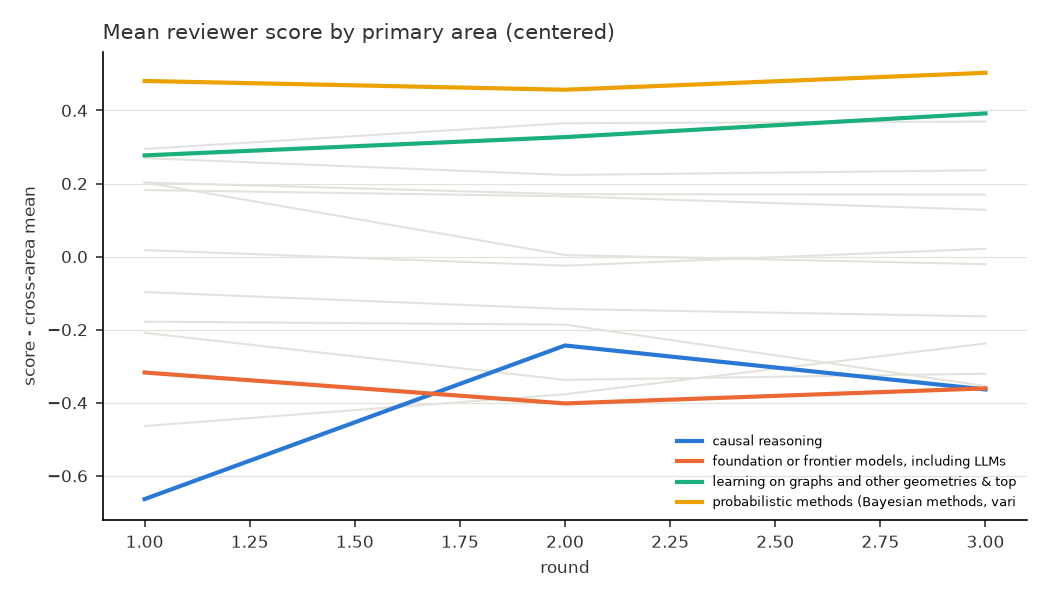
\includegraphics[width=.6\linewidth]{fig6_area_means.png}
\caption{Peer review (3 of 5 rounds, 194 papers). Top: homogenization metrics. Bottom: mean rating by primary area (centered); the four extreme areas are highlighted.}\label{fig:review}
\end{figure}

\section{Differences from the paper and limitations}
\begin{itemize}\itemsep1pt
\item \textbf{One model, one trial.} Every agent is Qwen3.8-27B; the paper's 16 mixed-model setups and 10-trial confidence intervals are not reproduced. Cross-trial variance and the code-similarity judge need $\ge2$ trials.
\item \textbf{Data.} Hiring job descriptions and r\'esum\'es are generated by Qwen3.8 itself (paper: Gemini) and use one signal variant per group (paper: five); the run uses 40 of 195 job descriptions. Stereotype directions come from BLS CPS Table~11 (ordering by over-representation, which the paper does not specify). For peer review OpenReview is not reachable, so papers come from public mirrors (PDFs text-extracted with PyMuPDF); withdrawn papers have no text available, so ``rejected/withdrawn'' is filled with rejected only.
\item \textbf{Ambiguities resolved by us.} Code reviewers see all earlier code and all reviewers' feedback (the paper's wording is ambiguous); the hiring adversary role rotates over the four evaluators by hashing the job description; unparsable replies are re-sampled twice and then dropped.
\item \textbf{Interpretation.} Score changes in code generation mix real quality improvement with homogenization; the paper's strict-inequality definitions also register ties at the scale ceiling as ``no change''.
\item \textbf{Not yet validated:} C/C++ CodeQL analysis.
\end{itemize}

\section{Reproduction}
Code and data live in \texttt{steering\_agents/}. Launch one job per application: \texttt{python scripts/launch\_mas\_pipeline.py --tier medium}; continue an interrupted run with \texttt{--resume <run\_dir>}; regenerate figures and tables with \texttt{scripts/analyze.py} and \texttt{scripts/quality\_report.py} (outputs in \texttt{<run>/analysis/}). The run described here is \texttt{experiments/medium\_20261026\_234912}; design notes are in \texttt{notes/plan.md}.

\nocite{h}
\begin{thebibliography}{9}
\bibitem{h} P.~Ganesh, K.~Wilson, L.~Zappella, B.-J.~Theobald, N.~Apostoloff, L.~Monteiro Paes, N.~Sivakumar. \emph{Homogenization in Multi-Agent Systems}. arXiv:2610.09824, 2026.
\end{thebibliography}
\end{document}
